\documentclass[12pt, letterpaper]{article}
\usepackage{amsmath,amsthm,amsfonts,amssymb,amscd}
\usepackage{fullpage}
\usepackage{lastpage}
\usepackage{enumerate}
\usepackage{fancyhdr}
\usepackage{mathrsfs}
\usepackage{listings}
\usepackage[T1]{fontenc}
\usepackage{xcolor}
\usepackage[margin=3cm]{geometry}
\usepackage{graphicx}
\renewcommand{\rmdefault}{ptm}
\setlength{\parindent}{0.0in}
\setlength{\parskip}{0.05in}

% Edit these as appropriate
\newcommand\course{CSE 573}
\newcommand\semester{Spring 2014}     % <-- current semester
\newcommand\hwnum{1}                  % <-- homework number
\newcommand\yourname{Shumo Chu} % <-- your name
\newcommand\email{chushumo@cs}           % <-- your CS login

\newenvironment{ans}[1]{
  \subsection*{Problem #1}
}%{\newpage}

\pagestyle{fancyplain}
\headheight 30pt
\lhead{\yourname\ (\email)\\\course\ --- \semester}
\chead{\textbf{\Large Problem Set \hwnum}}
\rhead{\today}
\headsep 10pt
\lstset{
    mathescape=true, 
    commentstyle={\color{gray}},
    numbers=left,
    xleftmargin=2em,
    frame=single,
    framexleftmargin=1.5em,
    basicstyle=\sffamily
    }

\begin{document}

\begin{ans}{1}
 \noindent \textbf{(a)}. 
 \begin{itemize}
    \item \textbf{State:} Let the $4$ gallon jug be $A$, the $7$ gallon jug be $B$. The state can be represented as the amount of water in each jug, namely $(W(A), W(B))$.
    \item \textbf{Initial State:} $(W(A)=0, W(B)=0)$
    \item \textbf{Goal Test:} The goal is reached when at least one of the following statement is true: $W(A)=2$ , $W(B)=2$
    \item \textbf{Actions:} 
        \begin{enumerate}
            \item Empty jug A: $W(A)\leftarrow 0$.
            \item Empty jug B: $W(B)\leftarrow 0$.
            \item Fill jug A: $W(A)\leftarrow 4$.
            \item Fill jug B: $W(B)\leftarrow 7$.
            \item Pour water from A to B.
            \item Pour water from B to A.
        \end{enumerate}
    \item \textbf{Cost:} The cost is accumualative along the path. Action 1., 2., 5. and 6. has no cost. The cost of action 3. or 4. is the amount of water that is actually filled.  
 \end{itemize}
 \noindent \textbf{(b)}. Figure~\ref{fig:prob1_bfs} shows the state diagram of breath first search. \emph{ea} and \emph{eb} represents emptying jub $A$ and $B$, respectively. \emph{fa} and \emph{fb} represents filling jug $A$ and $B$, respectively. \emph{pa} and \emph{pb} represents pouring water from jug $A$ and jub $B$ to the other jug, respectively. The all empty state and the all full state are ignored.
    \begin{figure}
        \centering
        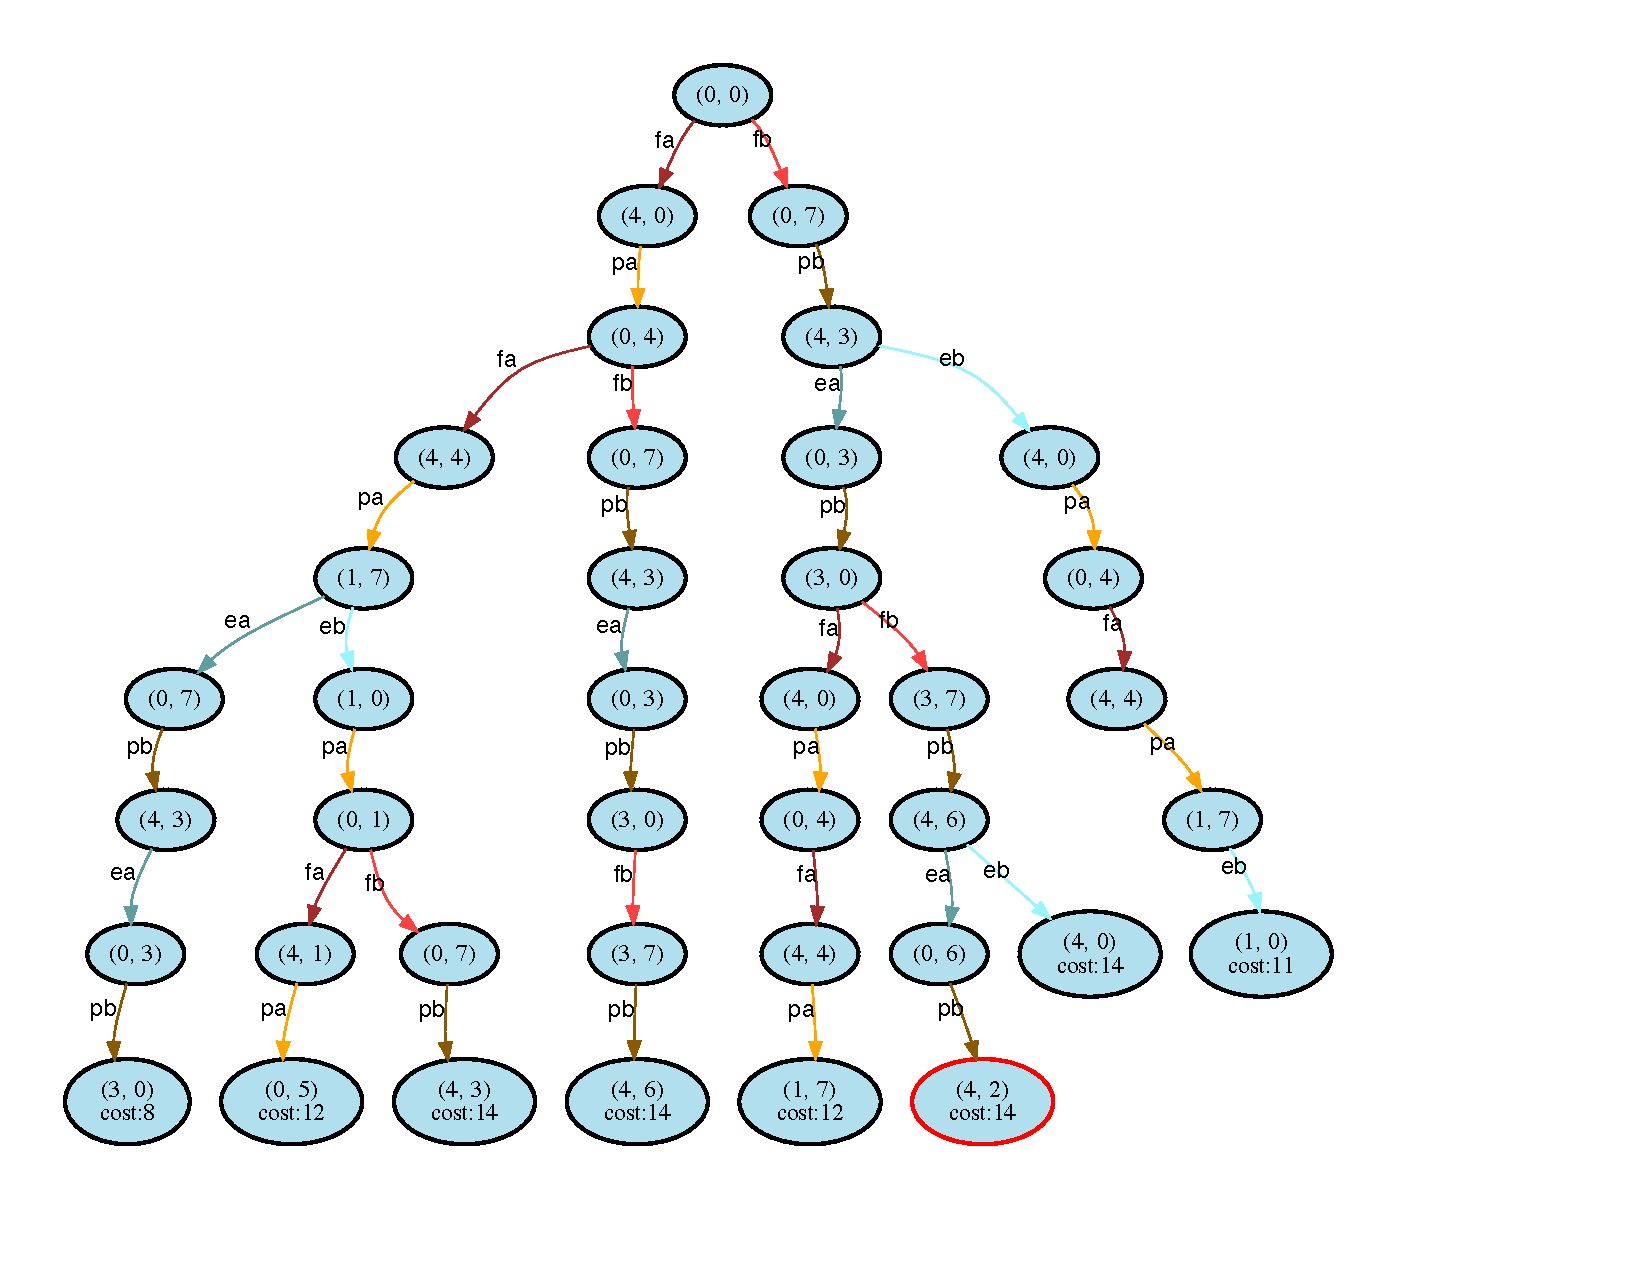
\includegraphics[width=0.99\textwidth]{tree}
        \caption{BFS state diagram of problem 1.}
        \label{fig:prob1_bfs}
    \end{figure}

 \noindent \textbf{(c)}. In this particular problem, it is optimal. We can verify this by checking the leaf nodes of tree. There are 4 nodes whose cost is smaller than the end node. However, they cannot reach the goal state with lower cost. For example, if we consider the leaf node $(3,0), cost:8$, we will find state $(3, 0)$ has appeared before on other branch of the search tree, it will need a \emph{fb} which add $7$ cost to reach the goal, thus it cannot be better than the result found. 

 In general, BFS may not be optimal unless the cost of each step is the same.

 \noindent \textbf{(d)}. The naive A* search will expand more nodes.

 Since the heuristic is always giving $0$ estimation, the A* will expand all the node on the order of current cost. One observation from Figure~\ref{fig:prob1_bfs} is that the end nodes has the larges cost among them. This means that if we use A*, more nodes with cost smaller than the end node will be expanded before reaching the end node.

\end{ans}

\begin{ans}{2}
\noindent \textbf{(a)}. The state can be represented by the locations of the $n$ vehicles. Since they are non-overlapping, the size of the state space is the number of unique arragement of the $n$ vehicles on the grid, which is $\prod_{i=1}^n {(n^2+1-i)}$.

\noindent \textbf{(b)}. Each vehicle can move $1$ in each direction, move $2$ in each direction (hop over) or stay. So the branching factor is at most $9^n$.

\noindent \textbf{(c)}. The following is an admissible heuristic. 
 \begin{equation}
    h_i = \frac{|x_i - (n-i-1)| + |y_i - n|}{2}
 \end{equation}
 Firstly, suppose the vehicle moves $1$ on each step, then the manhattan distance from its current position to the target is an admissible heuristic. Now the vehicle can at most moves $2$ on each step. This at most halves the number of steps.

 \noindent \textbf{(d)}. Suppose $h_i$ is any admissible heuristic for any $i$, then:
    \begin{enumerate}
        \item $\sum_{i=1}^{n}h_i$ may not be admissble. Here is a counter example. Let $n$ be 3, and we use the heuristic in \textbf{(c)}. It is easy to calculate that $h_1 = 2$, $h_2 = 1$ and $h_3 = 2$. Thus, $\sum_{i=1}^{n}h_i = 5$ . This estimate is not admissible since you can use $3$ steps to reach the goal: 
        \begin{enumerate}
          \item move $1$, $2$ and $3$ up; 
          \item move $1$, $2$ and $3$ up; 
          \item switch $1$ and $3$.
        \end{enumerate}
        \item $max(h_1,\ldots,h_n)$ is admissible. This can be proved by contradiction. Assume $max(h_1,\ldots,h_n)$ is not admissible, then there must be a vehicle, without the losing generality, $j$, which takes more step than $h_j$ reach its destination. This contradicts with the assumption that $h_j$ is admissible.
        \item $min(h_1,\ldots,h_n)$ is admissible. We have proved that $max(h_1,\ldots,h_n)$ is admissible. Since it is always true that $min(h_1,\ldots,h_n) < max(h_1,\ldots,h_n)$ , $min(h_1,\ldots,h_n)$ is admissible.
    \end{enumerate}

\end{ans}

\begin{ans}{3}
\end{ans}

\begin{ans}{4}
\end{ans}

\end{document}

